\setchapterimage[9cm]{headers/TDE_CloseUp_Landscape_01}
\setchapterpreamble[u]{\margintoc}
\chapter{AT2019dsg}
\labch{bran}
\begin{fquote}[Oscar Wilde][Lady Windermere's Fan][1893]We are all in the gutter, but some of us are looking at the stars
\end{fquote}

One key result of this thesis was the identification of a Tidal Disruption Event, \emph{AT2019dsg}, as a probable high-energy neutrino source. The object was found using the \ztf{} as part of our ZTF neutrino follow-up program, (see Chapter \ref{ch:ztf_too}), during a follow-up campaign for high-energy neutrino \emph{IC91001A} (see Chapter \ref{ch:realtime}). The association was first identified by the author, who led a multi-wavelength observation campaign to characterise this object. The data and analysis presented in this chapter are therefore the result of a collaboration between many people, not the sole work of the author. These results have also been published as a paper \sidecite{bran}.

\section{Observations of AT2109dsg}
\label{sec:bran_obs}

On 2019 October 1, the IceCube Neutrino Observatory reported the detection of a $\sim$0.2 PeV neutrino, IC191001A, with a 59\% probability of being of astrophysical origin \sidecite{stein:gcn25913} (see Chapter \ref{ch:realtime}). The event itself is shown in Figure \ref{fig:bran_eventview}. Seven hours later, the direction of the incoming neutrino was observed by ZTF as part of our neutrino follow-up program. The data was processed by the author's multi-messenger pipeline introduced in Chapter \ref{ch:ztf_too}, and the radio-emitting tidal disruption event AT2019dsg was identified as a candidate neutrino source \sidecite{2019ATel13160....1S}. 

\begin{figure}[!ht]
	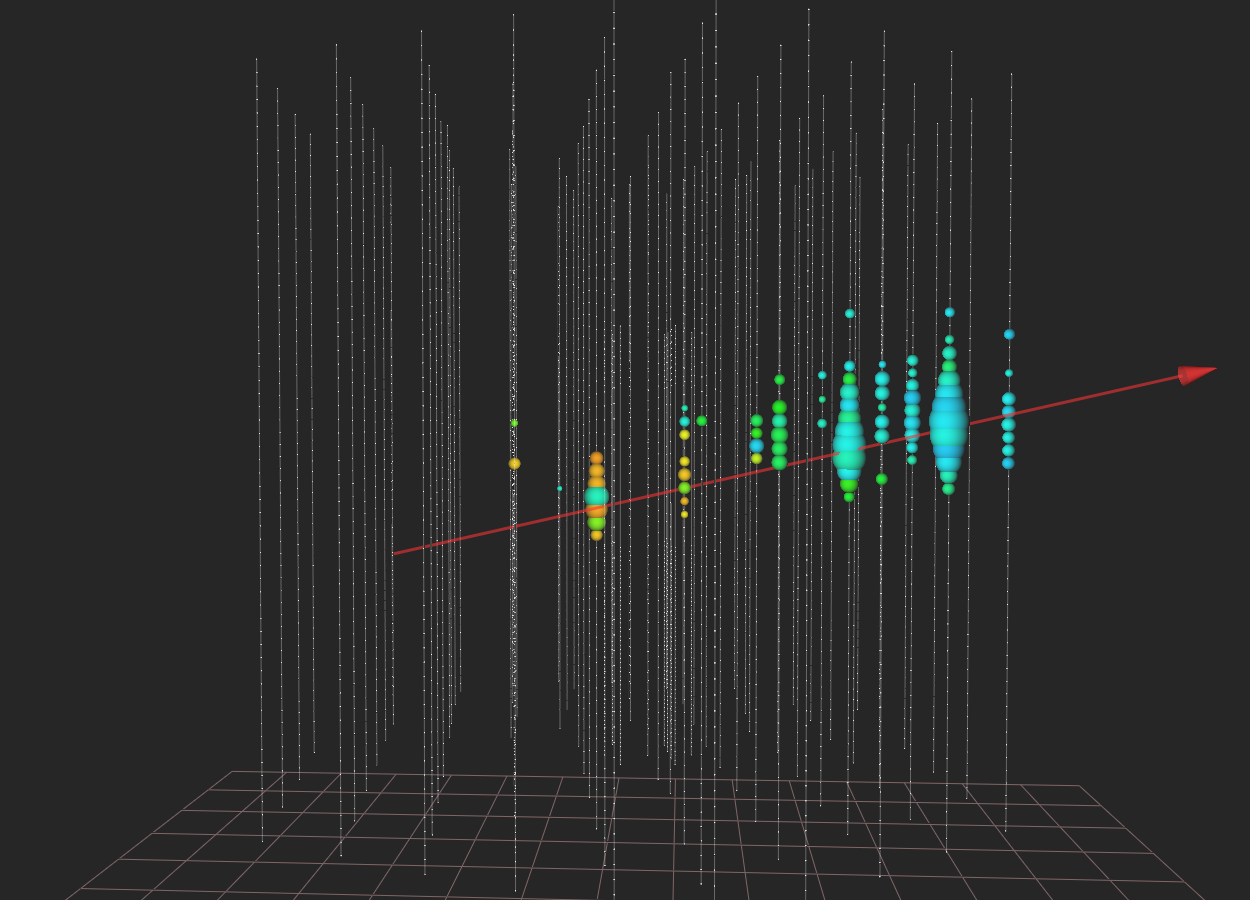
\includegraphics[width=0.8\textwidth]{Bran/bran_eventview}
	\caption{Visualisation of IC191001A in the IceCube detector. The colour corresponds to the light arrival time, from early orange pulses on the left to late blue ones on the right. The arrow illustrates the best fit reconstructed trajectory of the event.}
	\label{fig:bran_eventview}
\end{figure}

AT2019dsg (R.A.[J2000] = 314.26 deg, Dec[J2000] = +14.20 deg) was spatially coincident with the 90\% localisation of the neutrino IC191001A (R.A. = 314.08$^{+6.56}_{-2.26}$ deg,  Dec = +12.94$^{+1.50}_{-1.47}$ deg) \cite{stein:gcn25913}, at a distance of 1.27 deg to the best-fit position. It was also temporally coincident, being detected by ZTF in the ToO observations following the neutrino detection. There were additionally three candidate supernovae found in the error region of IC191001A, consistent with background expectations. 

AT2019dsg was the first TDE identified by our pipeline, and the first TDE to be reported in coincidence with any high-energy neutrino. As introduced in Chapter \ref{ch:neutrino sources}, TDEs have long been predicted as sources of neutrinos, where those TDEs with non-thermal emission are considered the most likely to be sources of high-energy neutrinos. Having already been detected at radio wavelengths, AT2019dsg was thus quickly identified as a promising candidate counterpart. The following subsections detail the electromagnetic observations of AT2019dsg, as published in \cite{bran}, but were not led by the author of this work.

\subsection*{UV/Optical Observations}

\begin{figure}[!ht]
	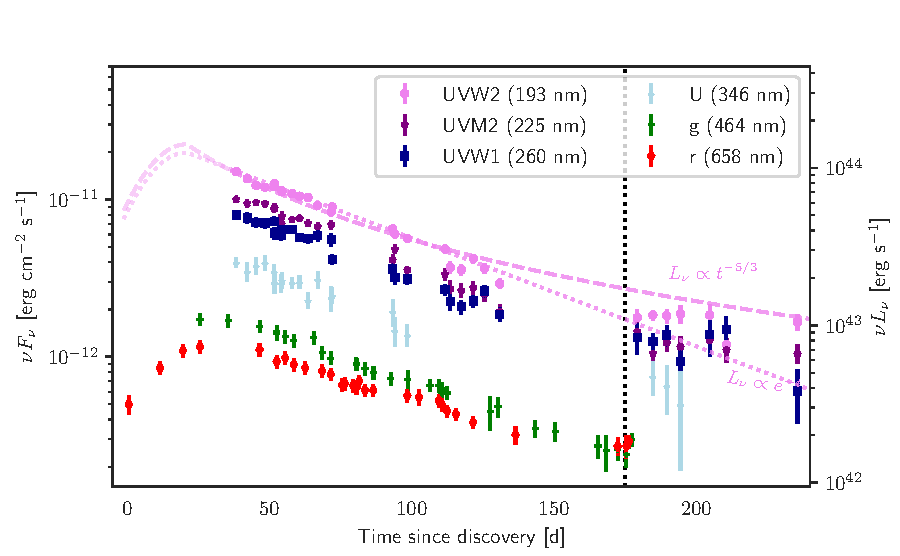
\includegraphics{Bran/uv_optical_lightcurve.pdf}
	\caption{UV/Optical photometry of AT2019dsg. The vertical dotted line illustrates the arrival of IC191001A.}
	\label{fig:bran_optical_lightcurve}
\end{figure}

AT2019dsg was first discovered by ZTF on 2019 April 9 \sidecite{2019TNSTR.615....1N}, and was had already been repeatedly detected by ZTF P48 telescope as part of the public MSIP survey prior to the detection of IC191001A.  These data were also supplemented by photometric observations from the 2m Liverpool Telescope \sidecite{2004SPIE.5489..679S} and SEDM \sidecite{Blagorodnova18} photometry obtained using the P60 telescope on Mt Palomar. AT2019dsg was selected as a probable TDE as part of a systematic search for optical TDEs with ZTF, each of which is assigned a nickname based on a character from HBO's TV Series \emph{Game of Thrones}, and was accordingly dubbed \emph{ZTF-BranStark} \sidecite{van_velzen_20}.

UV observations of AT2019dsg were conducted as part of a systematic survey of UV properties of all ZTF-identified TDEs \cite{van_velzen_20}, using the UltraViolet/Optical Telescope (UVOT) on board the \textit{Neil Gehrels Swift Observatory} (\textit{Swift}) \sidecite{2005SSRv..120...95R, 2004ApJ...611.1005G}. The first UV observation was performed 15 days after the optical peak on 2019 May 17, and a bright source spatially coincident with the TDE was detected. Subsequent observations continued at a cadence of 2--3 days, up to 2019 September 7. In this period, AT2019dsg continued to steadily dim. An additional observation occurred shortly before the neutrino detection on 2019 September 27. Follow-up observations were then triggered by the identification of a possible association with IC191001A, beginning on 2019 October 5. 

Like most TDEs \cite{van_velzen_20}, the optical/UV continuum of AT2019dsg was well described by a single blackbody photosphere. For AT2019dsg, this had an inferred radius of $10^{14.59 \pm 0.03}$~cm and a near-constant inferred temperature of $10^{4.59 \pm 0.02}$~K, with the latter being in the top 5\% of the 40 known optical TDEs to date \cite{van_velzen_20}. AT2019dsg was also particularly noteworthy for its high bolometric energy flux, the second highest of the ZTF sample. Not only was AT2019dsg relatively nearby for a TDE, but the peak luminosity of $10^{44.54 \pm 0.08}$ erg\,s$^{-1}$ was in the top 10\% of known optical TDEs \cite{van_velzen_20}. 

The late-time evolution, with an apparent UV plateau, is inconsistent with the canonical expectations for a steady power-law or exponential decay introduced in Chapter \ref{ch:sources}. However, this behaviour is compatible with the rapid formation of an accretion disk \sidecite{2020MNRAS.492.5655M}, which would be expected on these relatively short timescales for disruptions around higher-mass SMBHs. The total mass of the host galaxy of AT2019dsg is indeed in the top 10$\%$ of all optical TDEs, with an estimated black hole mass of $\sim 3 \times 10^{7} \Msol$ using a galaxy bulge scaling relation \cite{van_velzen_20}, further supporting this explanation. The source also appeared to redden in the optical bands at late times, a possible signature of reverberation due emission from TDE-heated dust which has been observed previously for some other objects \sidecite{2016ApJ...829...19V}. 

%\subsection*{Spectroscopy.}

\subsection*{X-ray Observations}

\begin{figure}[!ht]
	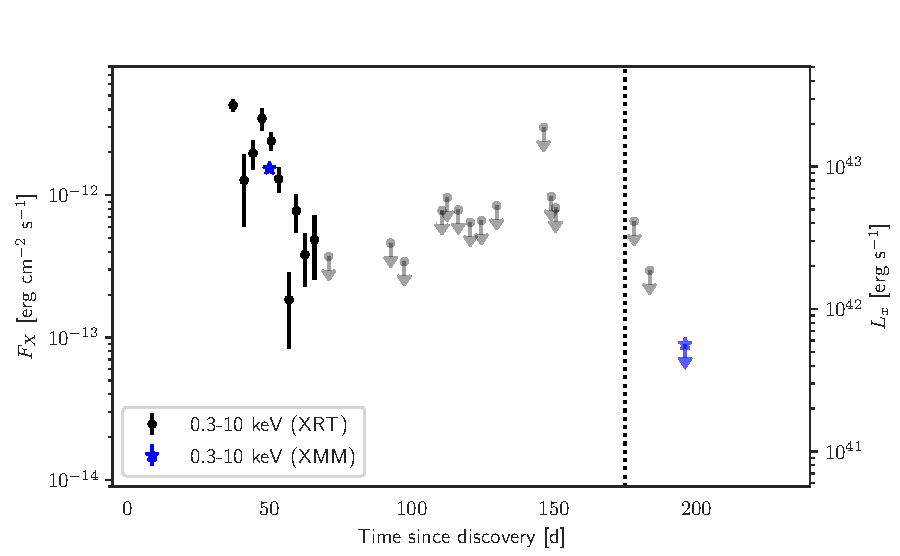
\includegraphics{Bran/xray_lightcurve.pdf}
	\caption{X-ray lightcurve of AT2019dsg. The vertical dotted line illustrates the arrival of IC191001A.}
	\label{fig:bran_xray_lightcurve}
\end{figure}

As shown in Figure \ref{fig:bran_xray_lightcurve}, AT2019dsg was also detected in X-rays beginning 37 days after discovery. It was first observed on 2019 May 17 by the X-Ray Telescope (XRT) \sidecite{2005SSRv..120..165B}, also on board \textit{Swift} \sidecite{2004ApJ...611.1005G}, as part of a program to categorise the X-ray properties of TDEs \cite{van_velzen_20}. Observations continued with a cadence of 2--3 days, and indicated a sharply-declining X-ray flux. One more sensitive observation was performed with the \textit{X-ray Multi-Mirror Mission} (\textit{XMM-Newton}) telescope \sidecite{2001A&A...365L...1J} on 2019 May 30, with the source clearly visible as seen in Figure \ref{fig:xraymap}. AT2019dsg was last detected by XRT on 2019 June 14, and not detected again in any of the following observations continuing until 2019 September 7. Following the identification of AT2019dsg as a candidate counterpart to IC191001A, additional X-ray observations were triggered but AT2019dsg was again not detected. An additional \textit{XMM} observation on 2019 October 23 yielded a deep upper limit of $9 \times 10^{-14}$ erg cm$^{-2}$ s$^{-1}$ (0.3--10 keV). 

\begin{figure}[!ht]
	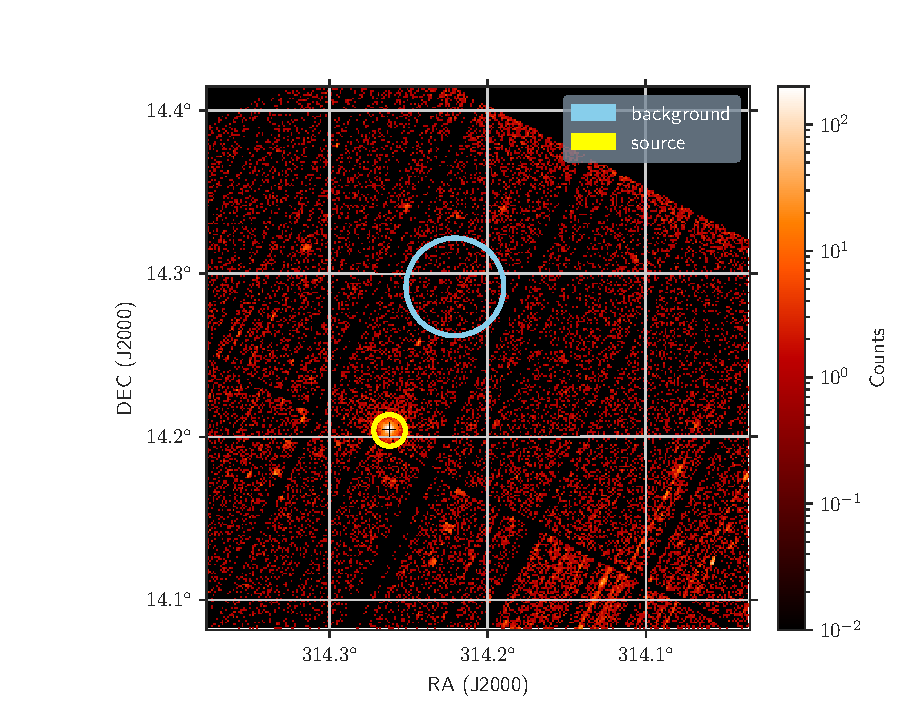
\includegraphics{Bran/extended_data_figure_2_xmm_countmap.pdf}
	\caption{X-ray count map from \textit{XMM-Newton} (50 days after discovery). The yellow circle indicates the source region, while the blue circular region was used to measure the background.}
	\label{fig:xraymap}
\end{figure}

Though the first X-ray observation indicated a bright source, with a high X-ray to optical ratio of $L_{\textup{X}}/L_{\textup{opt}} \sim $0.1, this X-ray flux faded extremely rapidly. This rate of decline is unprecedented, with at least a factor of 50 decrease in X-ray flux over a period of 159 days. Similar to the optical/UV emission, the observed X-ray spectrum was consistent with thermal emission, but from a blackbody of temperature $10^{5.9}$ K ($0.072 \pm 0.005$ keV) and, assuming emission from a circular disk, a radius $\sim 2 \times 10^{11}$ cm. This can be seen in Figure \ref{fig:xrayspec}. Since these X-ray observations probe close to the Wien tail of the thermal spectrum, the observed exponential decrease of the X-ray flux could simply be caused by cooling of the newly-formed TDE accretion disk \sidecite{2020MNRAS.492.5655M} , or it could instead result from increasing X-ray obscuration.

\begin{figure}[!ht]
	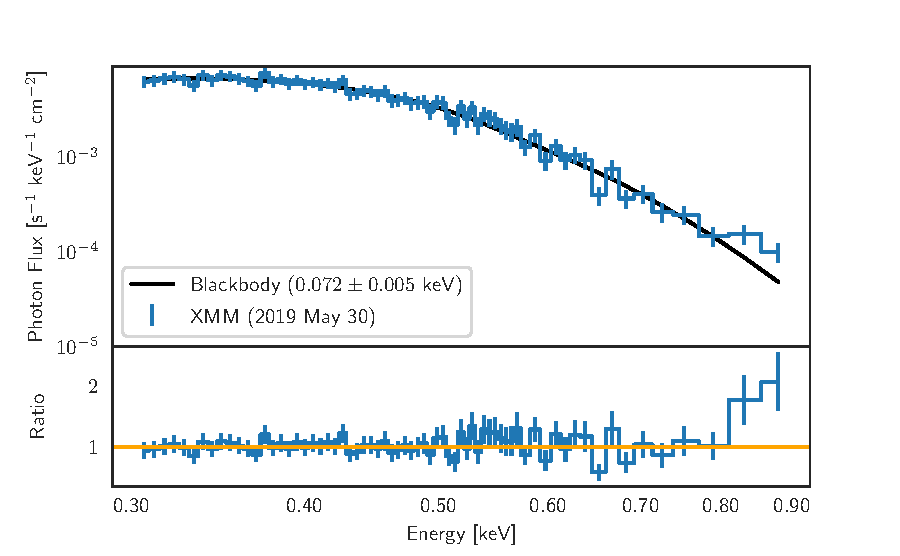
\includegraphics{Bran/extended_data_figure_3_xmm_spectrum.pdf}
	\caption{Soft X-ray spectrum of AT2019dsg measured by \textit{XMM-Newton}, fitted with an absorbed disk blackbody model.}
	\label{fig:xrayspec}
\end{figure}

As for most X-ray-detected TDEs, the blackbody radius appears much smaller than the Schwarzschild radius ($R_{\textup{S}} \sim 10^{13}$~cm) inferred from galaxy scaling relations \sidecite{2013ApJ...764..184M}.  Because X-ray emission is generally expected to arise close to the Schwarzschild radius, this inferred X-ray blackbody radius can be misleading. Small emitting areas can arise from an edge-on orientation, because the relativistic velocities at the inner disk can Doppler boost a large area of the disk out of the X-ray band.  Additionally, when extrapolating from the Wien tail behaviour, any decrease in inferred temperature due to unaccounted-for absorption would lead to a significantly underestimated blackbody radius and luminosity.

\subsection*{Radio Observations}

Quasi-simultaneous radio observations of AT2019dsg were conducted across a range of frequencies using the Karl G.\ Jansky Very Large Array (VLA) \sidecite{vla_11}, the AMI Large Array (AMI-LA) \sidecite{2008MNRAS.391.1545Z}, and the MeerKAT telescope \sidecite{meerkat}. These observations are shown in Figure \ref{fig:bran_radio}.  For all radio observations, the reported uncertainties include both the image background rms and a 5\% fractional calibration uncertainty, added in quadrature.

\begin{marginfigure}
	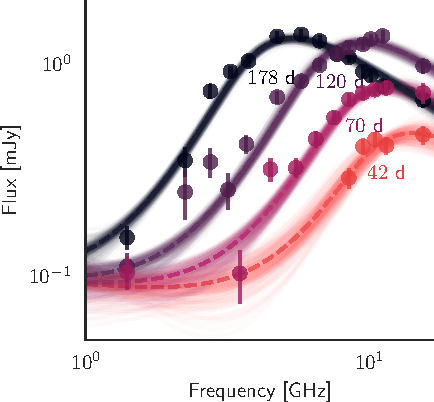
\includegraphics{Bran/radio_data.pdf}
	\caption{Radio observations of AT2019dsg.}
	\label{fig:bran_radio}
\end{marginfigure}

The four radio spectral energy distributions (SEDs) for AT2019dsg can be described by transient synchrotron emission from a population of relativistic electrons. It was assumed that the electrons are accelerated into a power-law distribution in energy $dN_{e}/d\gamma \propto \gamma^{-p}$. In addition to the transient radio emission from AT2019dsg, the observations also contain some steady radio emission from the host galaxy. This baseline flux density was parameterised as:

\begin{equation}\label{eq:Fhost}
F_{\nu, \textup{baseline}} = F_{ \textup{baseline}} \left(\frac{\nu}{1.28 \textup{ GHz}}\right)^{\alpha_{ \textup{baseline}}}
\end{equation}

such that the total flux density is given by :

\begin{equation}\label{eq:Ftotal}
F_{\nu,  \textup{tot}al} = F_{\nu \textup{baseline}} + F_{\nu,  \textup{sync}} 
\end{equation}

However, given the dramatic change in radio spectra between observation epochs, it is immediately clear that the majority of emission is indeed related to the transient rather than a steady host baseline. As outlined in Chapter \ref{ch:theory}, \emph{synchrotron self-absorption} will suppress the observed flux up to a threshold frequency, leading to a characteristic break in the synchrotron emission spectrum. This break is also clearly visible for each epoch shown Figure \ref{fig:bran_radio}. The intrinsic electron power law can be inferred from the \emph{optically-thin} (high-frequency) component of the spectrum, along with the break frequency itself (the \emph{synchrotron self-absorption frequency}).

%We expect that the lowest-energy electrons emit their synchrotron radiation below the synchrotron-self absorption frequency with negligible free-free absorption, and in this case the shape of the radio SED is determined by just 3 free parameters, the electron power-law index $p$, the magnetic field $B$ and the source radius $R$: 
%\begin{equation}\label{eq:Fsync}
%F_{\nu,  \textup{sync}}(t) \propto \frac{j_\nu(B(t), p)}{\kappa_\nu(B(t), p)} (1-e^{-\kappa_\nu R(t)})
%\end{equation}
%here $j_\nu$ and $\kappa_\nu$ are the emission and absorption coefficients, respectively. 
%

%The magnetic field and radius are allowed to change for each epoch, while $F_{ \textup{baseline}}$, $\alpha_{ \textup{baseline}}$ and $p$ are assumed to be constant during our radio observations. 
%
%Using Eq.~\ref{eq:Ftotal} to describe the synchrotron spectrum, 

A Markov chain Monte Carlo approach \sidecite{Foreman-Mackey13} was applied to determine a posterior probability distribution of the electron power-law index, as well as the peak frequency ($\nu_{ \textup{peak}}$) and peak flux density ($F_{ \textup{peak}}$) for each radio epoch. The measurement variance was allowed to be underestimated by some fractional amount $f$. The results are listed in Table \ref{tab:syncobs}. The resultant best fit is an electron spectrum with index $p = 2.9 \pm 0.1$, and a baseline with flux density $F_{\textup{ baseline}}=0.09\pm 0.01$ mJy and spectral index $\alpha_{\textup{baseline}} = -0.2\pm 0.1$, along with a best fit fractional error of $\ln f=-3.4$. No significant covariance was found between the baseline flux density parameters and the peak frequency or peak flux density. 

\begin{table}
	%\footnotesize
	\centering
	\begin{tabular}{| c| c c |}
		\hline
		$\Delta t$ & $F_{\textup{peak}}$ & $\nu_{\textup{peak}}$ \\ 
		  (days) & (mJy) &  (GHz)  \\
		\hline
		42 & $ 0.41\pm0.04$ & $ 14.8\pm1.0$ \\ 
		70 & $ 0.71\pm0.04$ & $ 12.0\pm0.5$ \\ 
		120 & $ 1.20\pm0.04$ & $  9.4\pm0.3$ \\ 
		178 & $ 1.24\pm0.04$ & $  5.4\pm0.1$ \\ 
		\hline
	\end{tabular}
	 \caption{Peak frequency and peak flux density of the radio observations.}
	\label{tab:syncobs}
\end{table}

%The last epoch of VLA observations, which has the best coverage of the optically thin part of the radio SED, yields $p=3.0 \pm 0.15$ and we use this as a Gaussian prior when fitting all data simultaneously.  We use a flat (uninformative) priors for the other parameters and we cap $\alpha_{\textup{baseline}}$ at 0 and $F_{\textup{baseline}}$ at 0.1 mJy (because the baseline flux density should be optically thin, $\alpha < 0$, and cannot exceed the observed post-TDE radio flux density). 
%
%For the time-independent parameters we find: $F_{\textup{ baseline}}=0.09\pm 0.01$ mJy, $\alpha_{\textup{baseline}} = -0.2\pm 0.1$, $p = 2.9 \pm 0.1$, and $\ln f=-3.4$. We find no significant covariance between the baseline flux density parameters and the peak frequency or peak flux density. 

Given the known distance to the source, and under particular assumptions about the source geometry, physical properties of the synchrotron-emitting region can be inferred from these data \sidecite{2013ApJ...772...78B}. The emission was modelled with a  conical geometry as expected for outflows (e.g., jets or winds) that are launched from---and collimated by---the inner parts of flared accretion disks that emit close to the Eddington limit. However these values depend critically upon assumed values for the so-called \emph{microphysical parameters} ($\epsilon_e$, $\epsilon_B$), where $\epsilon_e$ and $\epsilon_B$ respectively quantify the fraction of total energy carried by electrons and magnetic fields.  The derived values also depend on the electron power-law index, so the uncertainty on $p$ was propagated. 

One common assumption for such calculations is to assume \emph{equipartition}, where it is assumed that the system contains only electrons and magnetic fields. This yields a robust lower limit outflow energy, reached where $\epsilon_{e}/\epsilon_{B}=11/6$ \cite{2013ApJ...772...78B}, with any deviation from equipartition resulting in a higher total outflow energy. For the geometry of the outflow, the default model was two conical emitting regions with half-opening angles $\phi=$30\arcdeg. However, it should be noted that the opening angle for the outflow is largely unconstrained. The inferred equipartition properties of the source for $\phi=$30\arcdeg are given in the Table \ref{tab:sync_eq} for each epoch, alongside the corresponding values that would be derived for a spherical outflow.

\begin{table}
	\centering
	\begin{tabular}{|c | c | c c c c |}
		\hline
		&  & \multicolumn{4}{c|}{equipartition: $\epsilon_{e}/\epsilon_{B}=11/6$ (no protons)} \\
		&  $\Delta t$ & $R_{\textup{eq}}$ &  $E_{\textup{eq}}$ & $B_{\textup{eq}}$ & $n_{e, \textup{eq}}$ \\
		& (days)  &  (cm) & (erg) & (G) & (cm$^{-3}$) \\
		\hline
		\hline
		\multirow{4}{*}{\shortstack{Conical \\($\phi = 30\arcdeg $)}} 
		&  42& $16.29(0.02)$ & $47.9(0.1)$ &$-0.27(0.05)$ & $3.5(0.1)$\\
		&  70& $16.47(0.02)$ & $48.3(0.1)$ &$-0.36(0.04)$ & $3.3(0.1)$\\
		& 120& $16.68(0.02)$ & $48.7(0.1)$ &$-0.49(0.04)$ & $3.0(0.1)$\\
		& 178& $16.93(0.02)$ & $48.9(0.1)$ &$-0.73(0.05)$ & $2.6(0.1)$\\
		\hline     
		\multirow{4}{*}{\shortstack{Spherical}}
		&  42& $15.92(0.02)$ & $47.4(0.1)$ &$-0.00(0.04)$ & $4.0(0.1)$\\
		&  70& $16.10(0.02)$ & $47.8(0.1)$ &$-0.10(0.04)$ & $3.8(0.1)$\\
		& 120& $16.31(0.02)$ & $48.2(0.1)$ &$-0.22(0.04)$ & $3.6(0.1)$\\
		& 178& $16.56(0.02)$ & $48.4(0.1)$ &$-0.47(0.04)$ & $3.1(0.1)$\\
		\hline
	\end{tabular}
	\caption{Summary of the synchrotron modelling for the \emph{equipartition case}. All inferred properties are given in $\log_{10}$ scale, with errors given in brackets.}
	\label{tab:sync_eq}
\end{table}

Though the equipartition case provides a useful lower limit, it remains unrealistic as a central estimate because it neglects any contribution to outflow energy from protons. While our radio observations primarily probe electron emission, electrons are generally accelerated with much lower efficiency than protons in astrophysical accelerators  \sidecite{2012A&A...538A..81M}, so it is reasonable to assume that protons will actually carry a significant portion of energy. Motivated by observations of GRB afterglows \sidecite{Granot14,Fong15}, supernovae \sidecite{2013MNRAS.436.1258H} and the relativistic TDE Swift~J1644+57 \sidecite{2018ApJ...854...86E}, values of $\epsilon_e=0.1$ and $\epsilon_B=10^{-3}$ were assumed. The total estimated outflow energy, and other inferred properties for these assumptions, are given in Table \ref{tab:sync_fid}. These inferred energies are, as expected, substantially larger than for the equipartition case.

\begin{table}
	%\footnotesize
	\centering
	\begin{tabular}{|c | c | c c c c |}
		\hline
		&  &  \multicolumn{4}{c|}{proton model: $\epsilon_e=0.1$; $\epsilon_B = 10^{-3}$} \\
		&  $\Delta t$ & $R$ & $E$ & $B$ & $n_e$ \\
		& (days)  &  (cm) & (erg) & (G) & (cm$^{-3}$) \\
		\hline
		\hline
		\multirow{4}{*}{\shortstack{Conical \\($\phi = 30\arcdeg $)}} 
		&  42&$16.18(0.03)$ & $49.4(0.1)$ & $-0.68(0.05)$ & $4.4(0.1)$ \\
		&  70&$16.37(0.02)$ & $49.7(0.1)$ & $-0.78(0.04)$ & $4.2(0.1)$ \\
		& 120&$16.57(0.02)$ & $50.1(0.1)$ & $-0.91(0.04)$ & $3.9(0.1)$ \\
		& 178&$16.82(0.02)$ & $50.3(0.1)$ & $-1.16(0.04)$ & $3.4(0.1)$ \\
		\hline     
		\multirow{4}{*}{\shortstack{Spherical}}
		&  42&$15.81(0.03)$ & $48.8(0.1)$ & $-0.41(0.04)$ & $4.9(0.1)$ \\
		&  70&$16.00(0.02)$ & $49.2(0.1)$ & $-0.52(0.04)$ & $4.7(0.1)$ \\
		& 120& $16.20(0.02)$ & $49.6(0.1)$ & $-0.65(0.04)$ & $4.4(0.1)$ \\
		& 178&$16.45(0.02)$ & $49.8(0.1)$ & $-0.89(0.04)$ & $3.9(0.1)$ \\
		\hline
	\end{tabular}
	\caption{Summary of the synchrotron modelling with the inclusion of protons. All inferred properties are given in $\log_{10}$ scale, with errors given in brackets.}
	\label{tab:sync_fid}
\end{table}

The results in Table \ref{tab:sync_fid} revealed a third distinct spectral component, namely synchrotron emission from an extended synchrotron-emitting outflow. For a half-opening angle, $\phi$, of 30\arcdeg\ a radius of $R = 1.5 \times 10^{16}$ cm was found for the first epoch (41 days after discovery), increasing to $R = 7 \times 10^{16}$~cm shortly after the neutrino detection (177 days after discovery). These values are substantially larger than the inferred blackbody radii from UV/optical/X-ray observations, indicating a separate emission zone for the synchrotron radiation. The implied expansion velocity of the outflow is roughly constant at $v/c = \dot{R}/c = 0.12 \pm 0.01 $ during the first three epochs, with a significant ($>3\sigma$) acceleration to $v/c = 0.21 \pm0.02$ for the last epoch. These are the expansion velocities of the synchrotron-emitting region itself, so provide a lower limit to the velocity at the base of the outflow.  Indeed even the hotspots of relativistic jets from active galaxies that are frustrated by gas in their host galaxy are typically observed to have subrelativistic expansion velocities of $\sim0.1c$ \sidecite{2003PASA...20...69P}. 

\begin{marginfigure}
	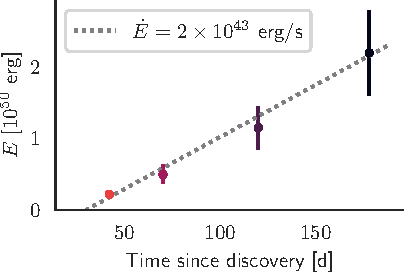
\includegraphics{Bran/outflow_energy.pdf}
	\caption{Inferred energy of the synchrotron-emitting outflow of AT2019dsg.}
	\label{fig:bran_energy}
\end{marginfigure}

\begin{marginfigure}
	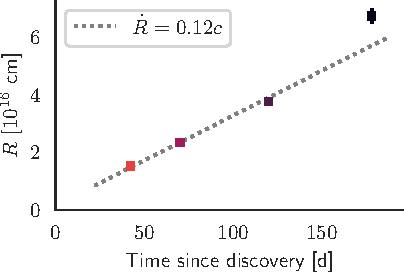
\includegraphics{Bran/outflow_radius.pdf}
	\caption{Inferred radius of the synchrotron-emitting outflow of AT2019dsg.}
	\label{fig:bran_radius}
\end{marginfigure}

The inferred outflow energy, $E$, shows a linear increase from $2.5 \times 10^{49}$~erg to $2 \times 10^{50}$~erg (Figure \ref{fig:bran_energy}), which would not be expected from models of TDE radio emission which involve a single injection of energy \sidecite{2016ApJ...819L..25A,2016ApJ...827..127K}. The constant increase of energy implies a constant injection rate at the base of the outflow, of approximately $2\times10^{43}$\,erg\,s$^{-1}$. While some scenarios can yield an increase in inferred energy from a single energy injection, none of these are consistent with the full set of observed properties. First, a single ejection with a range of velocities could explain the observed linear increase of energy with time (the slower ejecta arrive later), but is incompatible with the increasing velocity. Second, an increase of the efficiency for conversion of Poynting luminosity to relativistic particles is unlikely because the target density that is available to establish this conversion is decreasing.  And finally, an apparent increase of the inferred energy due to an increase of solid angle that emits to our line of sight is only expected for relativistic outflows that decelerate. Instead, for AT2019dsg, the observations suggest the presence of a central engine that yields continuous energy injection through a coupling of accretion power to the radio emission \sidecite{2018ApJ...856....1P}, with acceleration in the final radio epoch due to a decrease in the slope of the ambient matter density profile. 

There is, however, no evidence of correlation between the X-ray and radio emission in AT2019dsg. This is in contrast to coupling found for TDE ASASSN-14li \sidecite{2018ApJ...856....1P}. Such a correlation would only be expected if the X-ray luminosity of AT2019dsg served as a tracer of disk power, but the rapid observed fading indicates that the observed X-ray emission in AT2019dsg is instead driven either by varying obscuration or temperature evolution. 

%To estimate the radius and energy of the radio-emitting region from the posterior distribution of $F_{ \textup{peak}}$, $\nu_{ \textup{peak}}$, and $p$, we use the scaling relations from {Barniol Duran}, {Nakar}, \& {Piran} (2013) \cite{2013ApJ...772...78B}. These relations depend on the electron power-law index and we propagate the uncertainty on $p$ into our estimates of $R_{ \textup{eq}}$ and $E_{ \textup{eq}}$. Additional assumptions for the geometry and the microphysical parameters are required. For the geometry of the outflow, our default model is two conical emitting regions with half-opening angles $\phi=$30~deg, which yield an area covering factor $f_A=1-\cos \phi=0.13$ and a volume factor $f_V=2/(3\tan \phi )=1.15$ (here we follow the convention \cite{2013ApJ...772...78B} that $f_A=1$ and $f_V=4/3$ parameterise a spherical outflow in the Newtonian limit). 

%The equipartition energy, $E_{ \textup{eq}}$ is obtained under the assumption that the system contains only electrons and magnetic fields (both uniformly-distributed) and that the total energy is minimised for $E_{B} = (6/11)$ $E_{e}$. However we expect that protons carry the bulk of the energy and we parameterise this energy in protons by $\epsilon_e \equiv E_e/E_p$ with $E_p$ the total energy in relativistic protons.  After this adjustment, $E_{ \textup{eq}}$ is increased by $(1+1/\epsilon_e)^{11/(13+2p)}$. Finally, for systems that are not in equipartition, the energy is larger by a factor\cite{2013ApJ...772...78B} $(11/17) \eta^{-6/17} + (6/17) \eta^{11/17}$, with $\eta\equiv (\epsilon_B/(1-\epsilon_B))/(6/11)$, with $\epsilon_B$ the fraction of total energy that is carried by the magnetic field. Motivated by observations of GRB afterglows\cite{Granot14,Fong15}, supernovae\cite{2013MNRAS.436.1258H} and the relativistic TDE Swift~J1644+57\cite{2018ApJ...854...86E}, we use $\epsilon_e=0.1$ and $\epsilon_B=10^{-3}$. %For these parameters, the equipartition energy and radius are scaled by factors $25$ and 0.78, respectively, see Table~\ref{tab:syncinf}. 

%From the equipartition magnetic field strength inferred from the first epoch of radio observation (see Extended Data Figure 8) we estimate that the cooling time of the electrons that emit at 10~GHz is 500~days. For the last epoch, the field strength has decreased by a factor of 3 and now the cooling time is an order of magnitude longer. We can thus conclude that, unless the magnetic field energy density is much higher than the equipartition value ($\epsilon_B/\epsilon_e\gg1$), the observed slope of the optically thin part of the radio SEDs reflects the intrinsic power-law index of the electrons. 

\subsection*{Gamma-Ray Observations}

Gamma-ray observations were provided by the %pair-conversion telescope 
\textit{Fermi} Large Area Telescope (\textit{Fermi}-LAT) \sidecite{2009ApJ...697.1071A}, sensitive to gamma rays with energies from 20 MeV to greater than 300 GeV. During its sky-survey operations, the pair-conversion telescope \textit{Fermi}-LAT scans the entire sky every three hours, and can monitor the variable gamma-ray sky over short and long timescales. A search was performed within the 90\%\ error region during both the 1-day and 1-month period prior to the arrival of the high-energy neutrino, as part of a systematic LAT realtime neutrino follow-up program \sidecite{garrappa_buson:gcn25932}. No new gamma-ray source was identified, and there was no significant ($\geq 5 \sigma$) detection for any source from the fourth \textit{Fermi}-LAT point source catalog (4FGL \sidecite{2019arXiv190210045T}).

Following the identification of AT2019dsg as a candidate neutrino source, a dedicated point-source analysis centred on the object was then performed over three different time intervals under the assumption of a power-law spectrum. The duration of each interval was motivated by the multi-wavelength behaviour of the source. The first interval (G1) includes 130 days of observations that include the peak of the optical emission from 2019 April 4 to 2019 August 12. The second (G2) spans from 2019 August 12 to 2019 November 20 and covers the apparent UV plateau and the peak of the radio emission. The third interval (G3) integrates the whole period between the start of G1 up to 2020 January 31. No significant emission was found, as can be seen in Figure \ref{fig:fermi}. Upper limits were accordingly derived for the energy flux (integrated over the whole analysis energy range) have been derived for a power-law spectrum ($dN/dE \propto E^{-\Gamma}$) with photon power-law index $\Gamma$ = 2 and are listed in Table \ref{tab:lat_uls}, along with the respective time intervals.

\begin{figure}
	\centering
	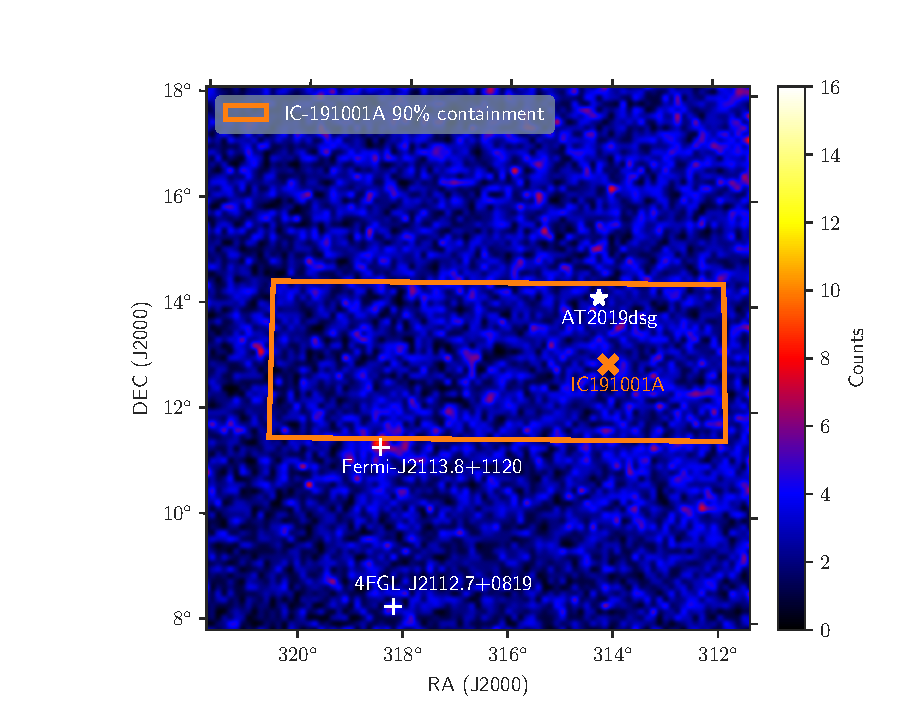
\includegraphics{Bran/lat_countmap.pdf}
	\caption{LAT counts map of the Region Of Interest (ROI) in the integrated search period G3, showing the IC191001A 90$\%$ localisation region in orange. The neutrino best-fit position is marked with a orange `$\times$'. %Gamma-ray sources significantly detected ($\geq$ 5 $\sigma$) are marked with white crosses. 
	}
	\label{fig:fermi}
\end{figure}

\begin{table}
	\centering
	\begin{tabular}{||c c c c||} 
		\hline
		\textbf{Interval} & \textbf{MJD Start} & \textbf{MJD Stop} & \textbf{UL}\\
		& & &  (erg cm$^{-2}$ s$^{-1}$)\\
		\hline
		\textit{G1} & 58577 & 58707 & 2.6 $\times 10^{-12}$\\
		\textit{G2} & 58707 & 58807 & 1.2 $\times 10^{-11}$\\
		\textit{G3} & 58577 & 58879 & 2.0 $\times 10^{-12}$\\
		\hline
	\end{tabular}
	\caption{Gamma-ray energy flux upper-limits for a point-source with power-law index $\Gamma$=2.0 at the position of AT2019dsg integrated over the analysis energy range 0.1-800 GeV.}
	\label{tab:lat_uls}
\end{table}

In all three time intervals, a new non-catalogued gamma-ray emitter was detected in the RoI at a significance $\geq 5 \sigma$. This source lies just outside the IC191001A 90$\%$ error region, as indicated in Figure \ref{fig:fermi}. The source, labelled \textit{Fermi}-J2113.8+1120, is likely the gamma-ray counterpart of the radio-loud object GB6 J2113+1121, classified as a flat-spectrum radio quasar with redshift $z = 1.63$ \sidecite{2013ApJ...767...14P}. The detection of an unrelated gamma-ray blazar within the neutrino uncertainty area is consistent with the background estimation. On average 1.5 4FGL gamma-ray blazars are expected in 20 sq.\,deg. A lightcurve analysis, shown in Figure \ref{fig:fermi_lc}, reveals that the source was last detected in gamma rays one month prior to the IC191001A detection, and was not significantly detected again until another month after the neutrino detection. This is compatible with the findings of the realtime follow-up of the region \cite{garrappa_buson:gcn25932}. Such a long apparent lag between gamma-ray emission and neutrino emission is disfavoured by recent studies on the temporal behavior of hadronic processes in blazars \sidecite{2015ApJ...802..133D,2019NatAs...3...88G}, suggesting that the blazar is unlikely to have produced the neutrino. There is thus no obvious connection between the gamma-ray observations of \textit{Fermi}-J2113.8+1120 and IC191001A.

\begin{figure}
	\centering
	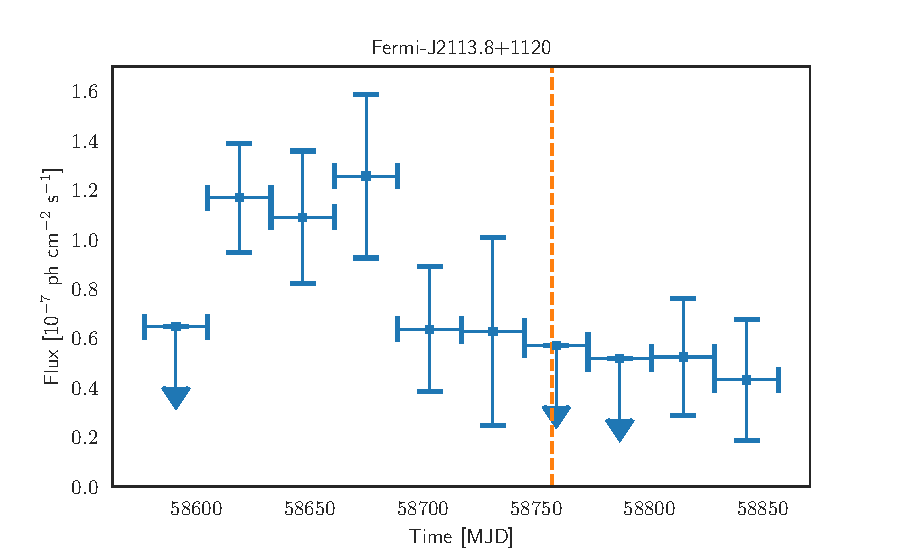
\includegraphics{Bran/fermi_lightcurve}
	\caption{LAT lightcurve for the source \textit{Fermi}-J2113.8+1120 in the time interval G3, with evenly spaced binning of 28 days. Vertical error bars represent 1$\sigma$ intervals, horizontal bars denote bin width. 2$\sigma$ upper limits are shown for bins with TS$\leq$9. The orange dashed vertical line marks the arrival time of IC-191001A.}
	\label{fig:fermi_lc}
\end{figure}

The HAWC observatory also reported a search for transient gamma-ray emission on short timescales in the localisation of IC191001A \sidecite{ayala:gcn25936}, and set an upper limit for their most significant position at 95\% confidence of $E^{2} dN/dE = 3.51 \times 10^{-13} (\textup{E}/\textup{TeV})^{-0.3}$ TeV cm$^{-2}$ s$^{-1}$, in the energy range 300 GeV to 100 TeV, for the period from 2019 September 30 05:46:52 UTC to 2019 October 02 06:03:29 UTC. We note that this search covered a relatively large region of the sky, and thus had a large associated trial factor. A dedicated search at the position of AT2019dsg would be more sensitive, especially one that additionally targeted the longer period over which the central engine is active.

\subsection*{Spectroscopy}

AT2019dsg was first classified as a TDE by ePESSTO+ on on 2019 May 13 \sidecite{2019ATel12752....1N}, and the redshift of AT2019dsg was measured to be $z=0.051$. This implies a luminosity distance $D_{\L} \approx$ 230 Mpc assuming a flat cosmology with $\Omega_{\Lambda}$ = 0.7 and $H_{0}$ = 70 km s$^{-1}$ Mpc$^{-1}$.  Further high-resolution spectroscopic observations were conducted using the De Veny Spectrograph on the 4.3m Lowell Discovery Telescope (LDT), the Kast Double Spectrograph on the 3m Lick Observatory Shane Telescope (Lick) \sidecite{Miller93}, and the Low Resolution Imaging Spectrograph on the 10m Keck Telescope (Keck) \sidecite{Oke95}, with the most recent spectrum on 2019 September 25. These spectra confirmed that AT2019dsg belonged to the common spectroscopic class of TDEs with Bowen fluorescence emission lines and broad H$\alpha$ emission lines \cite{van_velzen_20}. 

Following the identification of AT2019dsg as a candidate neutrino source, additional high-resolution spectra of the source were taken with the 200in Hale Telescope Double Spectrograph at Palomar Observatory (P200) on 2019 October 3 and again with  Lick on 2019 October 5 and 2019 October 29. As seen in Figure \ref{fig:bran_spectrum}, there is no evidence of any significant spectral evolution between these spectra and the most recent pre-neutrino spectrum from 2019 September 25, and the spectral evolution of AT2019dsg is consistent with that of other TDEs \cite{van_velzen_20}. 

\begin{figure*}[h!]
	\centering 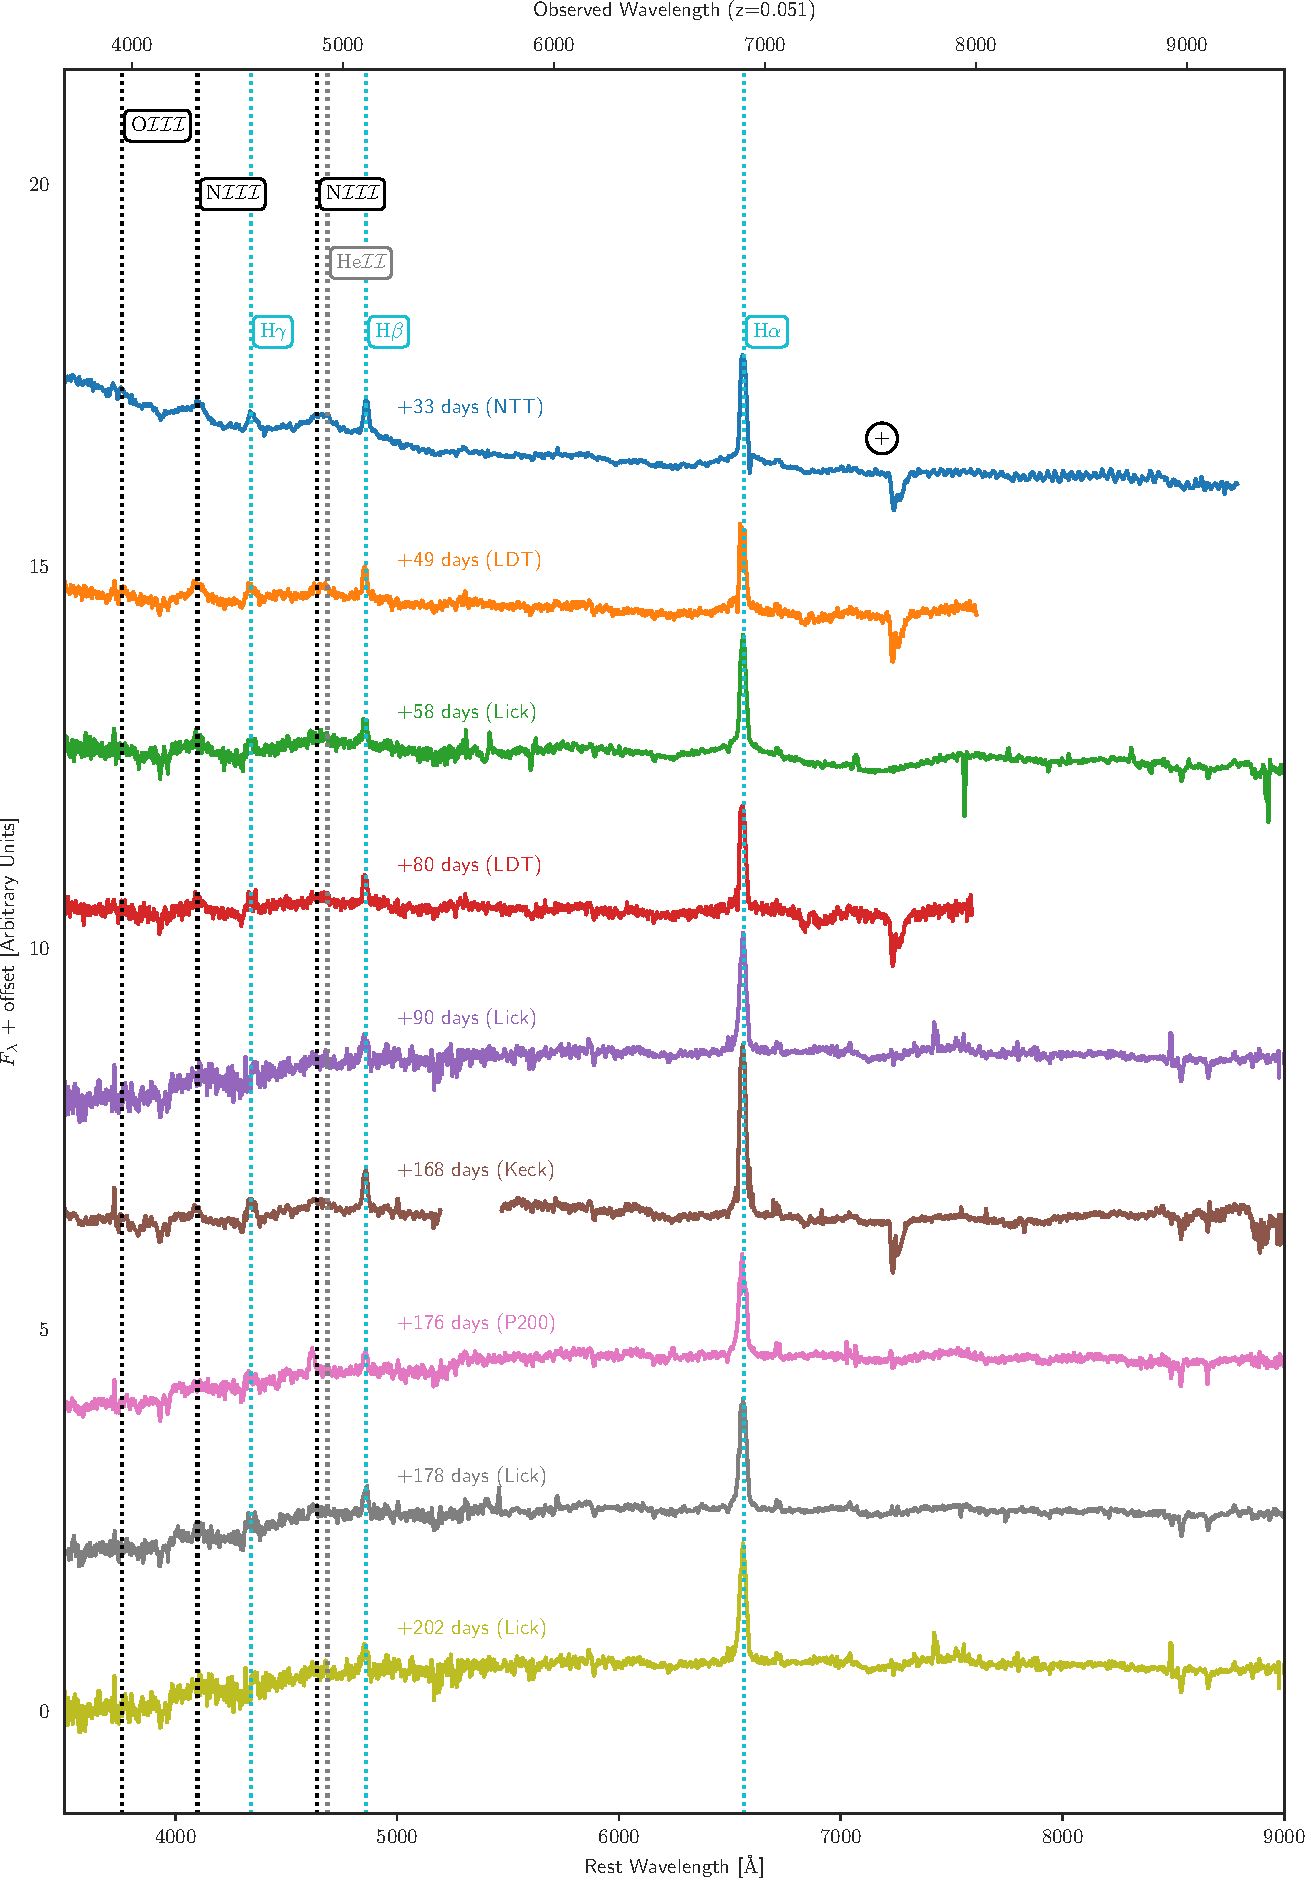
\includegraphics{Bran/edf1.pdf}
	\caption{The spectroscopic evolution of AT2019dsg, beginning with the publicly available classification spectrum taken with the NTT \cite{2019ATel12752....1N}, and further spectra from LDT, Lick, Keck and P200. The Balmer lines are highlighted in cyan, the HeII lines in gray, and the Bowen fluorescence lines (OIII at 3760\AA, NIII at 4100\AA ~and 4640\AA) in black. Telluric lines are marked with +.}
	\label{fig:bran_spectrum}
\end{figure*}

\section{Probability of Chance Coincidence}

One key question for the neutrino-TDE association is whether the observed coincidence is likely to have arisen merely by random chance. During the first 18 months of survey operations, ZTF identified 17 TDEs \cite{van_velzen_20}, distributed over 28000 deg of observed sky (the ZTF survey footprint, after removing sources with a Galactic latitude $|b|<7$). Of these TDEs, each was typically detected for $\sim$6 months\cite{van_velzen_20}. The density of ZTF-detected TDEs can thus be estimated as approximately 2.0 $\times 10^{-4}$ per sq.\,deg. of sky in the survey footprint at any given time. Our follow-up pipeline requires that any candidate be detected by ZTF in ToO observations following a neutrino, in order to establish temporal coincidence. We assume that our neutrino pipeline does not have a significantly higher selection efficiency than the dedicated ZTF program to identify TDEs \cite{van_velzen_20}, and thus that the latter provides a reasonable estimate on the background rate of TDEs passing our pipeline.

Those TDEs with radio detections are considered the most promising candidates for neutrino production, as the radio emission serves as a tracer for the particle acceleration required in neutrino sources. We can consider the fraction of TDEs which would additionally be detected in radio, assuming that all could be observed. Among the ZTF sample of confirmed TDEs, radio follow-up observations were undertaken with the VLA for 6, of which 2 were detected. Taking this implied radio-emitting fraction of 33\%, we find a final density of 5.9 $\times 10^{-5}$ radio-emitting TDEs per sq.\,deg. of surveyed sky. 

ZTF has followed-up eight neutrinos up to January 2020, and has covered a combined localisation region of 81.05 sq.\,deg (see Table \ref{tab:nu_alerts}). With this sky area, the expected number of coincident radio-detected TDEs across all of our neutrino follow-up campaigns is 4.8 $\times 10^{-3}$. The Poisson probability of observing at least one radio-emitting TDE during our entire neutrino follow-up campaign is thus 4.8$ \times 10^{-3}$. 

As radio follow-up observations of ZTF TDEs were biased towards those most likely to be detectable, this estimate is an overly conservative one. Because the bolometric energy flux derived from UV/optical observations (i.e., the blackbody luminosity over the square of the distance) serves as a proxy the non-thermal emission, TDEs which were bright under this metric were preferentially selected for radio observations. To avoid this selection bias, we can instead directly use this bolometric energy flux  as a proxy for neutrino flux to identify the most promising candidates for neutrino detection, namely those TDEs which are both nearby and luminous. Of the 17 TDEs observed by ZTF, AT2019dsg ranks second in this metric. The probability of finding a TDE in our neutrino follow-up campaign with a bolometric energy flux that is at least as high as AT2019dsg is thus 1.9$ \times 10^{-3}$. 

Like most other studies in neutrino astronomy \sidecite{2018Sci...361.1378I, ic_ps_10_yr}, these chance coincidence probability estimates do not account for the so-called ``look-elsewhere effect" from multiple possible hypotheses. In our case, the ZTF program has sensitivity to four theoretically-motivated neutrino population hypotheses (TDEs, core-collapse supernovae, gamma-ray bursts and AGN flares) \sidecite{2019PASP..131g8001G}. The impact of the testing multiple hypotheses is thus modest, and a chance coincidence explanation for AT2019dsg-IC191001A remains unlikely.

Of these four, it should also be noted that TDEs are the one to which our program is most sensitive. As introduced in Chapter \ref{ch:neutrino_cosmology}, follow-up programs are generally most effective in identifying neutrino emission from TDEs, since this flux should be dominated by nearby sources which can be detected by telescopes such as ZTF. Moreover, given their low rate, any individual TDE-neutrino association will be easier to identify than for more abundant populations such as AGN or supernovae. TDEs also evolve sufficiently slowly to enable extensive photometric and spectroscopic follow-up, in marked contrast to fast transients such as GRB afterglows, leading to a higher detection efficiency.

While an atmospheric origin  for the IC191001A-AT2019dsg association cannot be excluded, the improbability of chance temporal and spatial coincidence substantially reinforces the independent energy-based evidence of an astrophysical origin for IC191001A, and indicates that any atmospheric origin is unlikely.

\section{Neutrino production in AT2019dsg} 

\begin{figure}[!ht]
	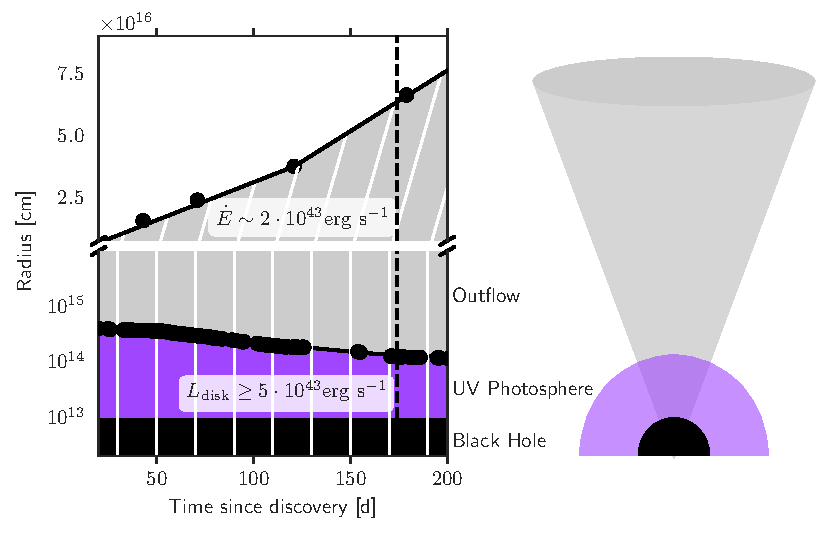
\includegraphics{Bran/figure_3_diagram.pdf}
	\caption{Left: temporal evolution of the three emission zones for AT2019dsg. Right: Illustration of the geometry of these three zones.}
	\label{fig:bran_diagram}
\end{figure}

Given that an atmospheric origin for IC191001A is unlikely, we can instead consider whether it is realistic for AT2019dsg to be the source of neutrino IC191001A. There are several requirements that an object must satisfy to be a neutrino source. In particular, neutrino production requires hadrons to be accelerated to sufficiently high energies, and to collide with a suitably abundant target. As demonstrated in Section \ref{sec:bran_obs}, there is strong evidence derived purely from multi-wavelength observations for the existence of three distinct emission zones in AT2019dsg, illustrated in Figure \ref{fig:bran_diagram}. 

% Accounting for the large Eddington bias that arises from the Poisson-dominated emission of single high-energy neutrinos\cite{2019A&A...622L...9S}, the TDE should reasonably have sufficient flux to produce an expected number of high-energy neutrino alerts $N_{\nu} \sim$ 0.01-1. 

Radio observations confirm that particle acceleration is indeed occurring, and that this continues without decline through to the detection of the neutrino at $\sim$180 days post-discovery. Given that neutrinos typically take a fraction $\eta_{p\nu} \sim 0.05$ of the parent proton energy, our accelerator must be capable of accelerating protons to at least 4 PeV. We evaluate the Hillas criterion \sidecite{1984ARA&A..22..425H} introduced in Equation \ref{eq:hillas} of Chapter \ref{ch:theory}, that the proton Larmor radius be less than the system size, to determine whether this is possible:

\begin{equation}
\frac{E_{ \textup{max}}}{ \textup{PeV}} \approx
1600 \times \frac{B}{ \textup{Gauss}} \times \frac{R}{10^{16} \,  \textup{cm}} \times
\beta Z
\end{equation}

We use our estimates for conditions in the synchrotron zone at the time of neutrino detection, with $B \sim$ 0.07 G and $R \sim 7 \times 10^{16}$ cm for the near-contemporaneous radio epoch. Taking this as a baseline, we find a maximum proton energy of $\sim$160 PeV, far in excess of our requirements. The Hillas criterion can also be satisfied within the engine that powers the radio-emitting outflow because the product $BR$ is not expected to decrease at smaller radii (e.g. $B \propto R^{-1}$ for a toroidal configuration). 

In order for particle acceleration to occur up to these energies, the timescale required for particle acceleration must also be shorter than the associated particle cooling timescale. Previous work has found this condition can be satisfied in TDEs for relevant energies \sidecite{2017ApJ...838....3S, 2017PhRvD..95l3001L}, although a detailed calculation is beyond the scope of this thesis.

Assuming that protons are indeed accelerated to sufficient energies, these must then collide with a suitably abundant target. For neutrino production, this can be either photons (p$\gamma$ interactions) or protons (pp interactions). For a photon target, neutrino production occurs above an energy determined by the mass of the $\Delta$ resonance. This threshold, as introduced in Equation \ref{eq:delta_res} of Chapter \ref{ch:theory}, can be approximated as:

\begin{equation}
E_{\gamma}E_{p} \sim \Gamma ^{2} 0.16 \,  \textup{GeV}^{2}
\end{equation}  

Substituting $E_{\nu} = \eta_{p\nu} E_{p}$ where again $\eta_{p\nu} \sim 0.05$ and $E_{\nu}$ is the energy of a single neutrino, this can then be translated into a threshold photon energy:

\begin{equation}
\frac{E_{\gamma}}{\textup{eV}} \gtrsim \left(\frac{\Gamma}{1} \right )^{2} \left(\frac{\eta_{p\nu}}{0.05} \right) \left( \frac{8 \textup{PeV}}{E_{\nu}} \right)
\end{equation}  

%For a thermal spectrum, of temperature $T$, we then find a corresponding neutrino energy $\epsilon_{\nu} $ of:

%\begin{equation}
%\epsilon_{\nu} \sim \eta_{p\nu}[(m_{\Delta}^{2} - m_{p}^{2})/ 4 \epsilon_\gamma ] \approx 0.3 \times \left( \frac{T}{10^{5} \textup{K}} \right)^{-1} \textup{PeV}
%\end{equation}

With this constraint, we can derive the necessary photon energies required for a target to produce IC191001A. Taking the reconstructed neutrino energy of $\sim$0.2 PeV directly, we find a threshold photon target of $E_{\gamma} \gtrsim $40 eV. However, these reconstructed neutrino energies typically have upper bounds an order of magnitude or more above the central estimate \sidecite{2018Sci...361.1378I}, so the true neutrino energy could be substantially higher. For example, with a true neutrino energy of $\sim$1 PeV, we would instead require photons $E_{\gamma} \gtrsim $8 eV for pion production.  In principle, this suggests that both UV and X-ray photons would be suitable targets.

We can then consider whether these photons are suitably abundant for efficient pion production. We can derive the mean free path, $\lambda$, for a proton:

\begin{equation}
\lambda = \frac{1}{\sigma_{p\gamma} n_{\gamma}}
\end{equation} with cross section $\sigma_{p\gamma} \sim 5 \times 10^{-28}$ cm$^{2}$ and photon number density $n_{\gamma}$. For the UV photosphere with a blackbody of temperature $T_{BB} \sim 10^{4.6}$ K, the mean free path for the parent proton of a 1 PeV neutrino is $\lambda \sim 2 \times 10^{13}$ cm. Accounting for the fact that each proton interaction will lead to a typical energy reduction of 20\%, we then find:

\begin{equation}
f_{\pi}(x) = 1 - e^{\left( \frac{-0.2x}{\lambda} \right)}
\end{equation} for path $x$, where $f_{\pi} \leq1$ is the conversion efficiency from total energy in protons, $\epsilon_{p}$, to total energy in pions, $\epsilon_{\pi}$, such that $\epsilon_{\pi} = f_{\pi} \epsilon_{p}$. Equating $x$ with the radius of the UV photosphere $x \approx 10^{14.6}$cm, we then find that each proton or neutron will typically undergo $\sim$ 10 interactions, which would represent a high efficiency $f_{\pi} \sim 0.9$, so the UV photosphere is indeed optically thick. At smaller radii, the X-rays would overtake the UV photons as dominant scattering targets. We caution that this estimate is only approximate, and that detailed numerical simulations are required to accurately calculate the pion production efficiency \sidecite{2010ApJ...721..630H}.

%For the UV photosphere, we find $\epsilon_\nu \sim$ 0.8 PeV, while for the compact X-ray source, we find $\epsilon_\nu \sim$ 0.05 PeV. Both of these values are compatible with the observed neutrino energy and uncertainty, so either photon field could serve as a target. 

It is however clear that conditions in AT2019dsg are sufficient for pion production to occur. A further requirement for the association is that there are sufficient neutrinos produced at the source for the detection of one high-energy neutrino like IC191001A to occur. During pion production roughly half of the energy will be lost through the neutrino-less $\pi^{0}$ channel \cite{2010ApJ...721..630H}, while for the charged pion channel energy is shared roughly equally among the decay products $\pi^{\pm} \rightarrow e^{\pm} + \overset{\brobor}{\nu_{e}} + \overset{-}{\nu_{\mu}} + \nu_{\mu}$ \sidecite{Waxman:1998yy}. Thus $\sim$3/8 of the pion energy is transferred to neutrinos, with a 1:2:0 flavour composition at source. However, as introduced in Chapter \ref{ch:theory}, neutrino oscillations across the cosmological baseline travelled will lead to a mixed 1:1:1 composition on Earth. The IceCube realtime event selection is dominated by muon neutrinos, a channel which will then carry no more than $\sim$1/8 of the pionic energy. Thus we find:

\begin{equation}
\epsilon_{\nu} \approx f_{\pi} \frac{\epsilon_{p}}{8}
\label{eq:pion_eff}
\end{equation} 

where $\epsilon_{\nu}$ is the total energy carried by muon neutrinos. We can calculate the effective area for a single high-energy neutrino. Below 1 PeV, this corresponds to an approximately-constant threshold of $6 \times 10^{-4}$ erg cm$^{-2}$ for an expectation of one neutrino alert. Given the redshift of AT2019dsg, we find a required total energy in neutrinos $\epsilon_{\nu} \approx 4 \times 10^{51}$ erg to produce a single neutrino alert. 
%With the assumed baryon loading ratio and beaming fraction, 
Approximating the sharply-peaked p$\gamma$ neutrino spectrum as a monoenergetic flux anywhere between  0.2 PeV $\lesssim E_{nu} \lesssim 1$ PeV, we can use Equation \ref{eq:pion_eff} to express the expected number of detected neutrinos as:

\begin{equation}
N_\nu \approx  \left(\frac{\epsilon_{\nu} }{E_\nu}\right)\left(\frac{A_{  \textup{eff}}} {4\pi D_{  \textup{L}}^{2}}\right) \approx 3 \times \frac{f_{pi}}{0.9} \times \frac{\epsilon_{p}}{10^{53}  \textup{erg}} 
\end{equation} 

This expectation would also be valid for any power-law distribution in the same energy range, assuming a similarly high pion conversion efficiency $f_{\pi}$. To obtain the expected number of neutrino alerts from this source we have to estimate the energy carried by protons ($E_{\textup{p}}$) that are accelerated above the energy threshold needed to produce high-energy neutrinos. The outflow energy of $2 \times 10^{50}$~erg derived from the radio observations (Table~\ref{tab:sync_fid}) represent a lower bound to the energy that is available for particle acceleration in a central engine.  Indeed, the total energy budget for a TDE is set by the mass of the disrupted star, with $\epsilon_{\textup{TDE}} \sim (1/2)\, 0.1 \, \Msol \, c^{2} \sim 10^{53}$ erg for a solar-mass star. We will assume 1\% of this total energy budget is carried by relativistic protons, $\epsilon_{\textup{p}} \sim 10^{51}$ erg. We then find $N_\nu \approx 0.03$, a number that remains less than unity for any reasonable assumption of $\epsilon_{p}$. 

However, this is not necessarily in tension with the IC191001A-AT2019dsg association, because the detection of a single high energy neutrino does not imply that a  single source must have a neutrino alert expectation of $\sim$1 \sidecite{2019A&A...622L...9S}. Rather, after accounting for Poisson counting uncertainty, the detection of a single high-energy neutrino such as IC191001A implies a mean expectation in the range $0.05 < N_{\nu, \textup{tot}} < 4.74$ at 90\% confidence where $N_{\nu, \textup{tot}}$ is the cumulative neutrino expectation for all TDEs that ZTF has observed. For an individual TDE the expectation will then be significantly lower. AT2019dsg emits $f_{\textup{bol}} \sim 0.16$ of the population bolometric energy flux, and if we take this as a proxy for neutrino emission, we would expect $0.008 \lesssim N_{\nu} \lesssim 0.76$ for this source assuming that conditions are similar in other ZTF TDEs. In that case, any optically-thick p$\gamma$ scenario would be sufficient for AT2019dsg to produce IC191001A. 

In the multi-zone model, shown in Figure \ref{fig:bran_diagram}, the thermal photons thus provide a guaranteed target for pion production. However hadrons could in principle also serve as a target, leading us to consider a single-zone scenario in which the protons are accelerated at the same location as the synchrotron-emitting electrons, with the neutrino spectrum following the same intrinsic energy power law as the protons and electrons. For pp neutrino production, high target densities of $n_{\textup{p}}\sim 1/(\sigma_{\textup{pp}} R)\sim 10^8$~cm$^{-3}$ would be required for efficient production of pions, where $\sigma_{\textup{pp}}$ is the proton-proton cross section and $R \sim 10^{17}$~cm is the characteristic size of the synchrotron-emitting region at the time of neutrino production. The synchrotron analysis provides an estimate of the number density of relativistic electrons, which in turn yields a lower limit to the total particle density in the radio region. For the energy and radius of last radio epoch, which was obtained a few days after the neutrino detection, we find an electron number density of $10^{3.4\pm 0.1}$~cm$^{-3}$ (see Table \ref{tab:sync_fid}). It is expected that the proton number density should be higher, owing again to the more efficient acceleration of protons than electrons \cite{2012A&A...538A..81M},  but the exact value is largely unconstrained.

The high required proton density could in principle be provided by the unbound stellar debris from the tidal disruption itself, although this component moves with a typical maximum velocity of $0.05\,c$ \sidecite{2016ApJ...827..127K}, so the majority of this debris would need to have been swept up with the outflow. Alternatively, the density could be provided by pre-existing gas in the galaxy core, though it would be challenging to avoid accompanying signatures of pre-TDE accretion. More critically, in contrast to a peaked p$\gamma$ neutrino spectrum, for pp production the neutrinos would instead follow a power law. Many of these neutrinos would then fall below the threshold of IceCube's alert selection, resulting in a lower $N_{\nu}$

Following the publication of the coincidence, multiple theoretical works have independently suggested possible models for neutrino production in AT2019dsg. Motivated by the unusual X-ray-bright nature of the source at early times, one suggested mechanism for the association is an obscured relativistic jet in AT2019dsg \sidecite{winter21_bran}. In that scenario, the X-ray emission is assumed to continue at late times, providing target photons. Ultimately an $N_{\nu} \approx 0.05$ was calculated, which would again be compatible with the observed association. An alternative explanation invoked a relativistic jet that was viewed somewhat off-axis (10-30\arcdeg) for which optical/UV photons instead serve as a target \sidecite{liu21_bran}. Such a model can produce $N_{\nu} \gtrsim 0.01$ without violating the gamma-ray constraints introduced in Section \ref{sec:bran_obs}, providing another viable explanation. A third suggested explanation did not invoke a relativistic jet, instead favouring an AGN-like corona model for neutrino production with proton acceleration through plasma turbulence or magnetic reconnection \sidecite{murase20_bran}. Under optimistic assumptions such a scenario would be a possible explanation, yielding a sufficient $N_{\nu} \approx 0.01$.

Given these many different possible neutrino spectrum expectations, a search for accompanying lower-energy neutrinos could be used to probe the conditions at the site of proton interaction. As reported in Chapter \ref{ch:results}, such a search was conducted as part of this thesis for an older sample of TDEs, but no such IceCube analysis has yet been performed for AT2019dsg. 

An analysis was published by the ANTARES collaboration, and did not find any significant excess of neutrino emission from AT2019dsg \sidecite{antares_at2019dsg_21}. A time-integrated search was performed from the date of ZTF TDE discovery, 2019 April 9, up to 2020 February 29. A muon neutrino upper limit was set of $1.0 \times 10^{−7}$ GeV$^{−1}$ cm$^{−2}$ s$^{−1}$ for an E$^{-2}$ spectrum in the range 4 TeV - 4 PeV, corresponding to a fluence upper limit of 19 GeV cm$^{−2}$ or 0.03 erg cm$^{−2}$. For such an E$^{-2}$ power law, the energy is distributed:

\begin{equation}
	\frac{dN_{\nu}}{dE} = \phi_{0} \left(\frac{E}{E_{0}} \right) ^{2}
\end{equation}

\begin{equation}
\epsilon_{\nu} = \int^{E_{max}}_{E_{min}} E \frac{dN_{\nu}}{dE} dE = \phi_{0} E_{0}^{2} \left(\ln(E_{max}) - \ln({E_{min}})\right)
\end{equation}

The neutrino energy range of 0.2-1 PeV to which IceCube alerts are most sensitive to should carry 23\% of the total energy in this range for an E$^{-2}$ power law, corresponding to a fluence of $7 \times 10^{-3}$ erg cm$^{−2}$. This limit is then a full order of magnitude greater than the flux required to produce a single high-energy neutrino alert in this energy range in IceCube, and far in excess of all reasonable predictions for neutrino emission in AT2019dsg. The ANTARES non-detection is thus not constraining for the scenarios outlined above, and not in tension with an association between IC191001A and AT2019dsg.

\section{Compatibility with stacking limit}
\label{sec:diffuse}

We can further estimate the contribution of TDEs to the diffuse neutrino flux that would be required to produce an observation of one association with our ZTF follow-up program. As outlined in Table \ref{tab:nu_alerts}, a total of eight neutrino alerts were observed through to January 2020. For all but one of these, IceCube reported an estimate of the \emph{signalness}, i.e., the probability for each to be astrophysical. It should be noted that this quantity is not an absolute value, but is rather derived under specific assumptions about the underlying neutrino source population. Nonetheless, if these estimates are taken at face value, and it is assumed that the additional event had the a signalness equal to the mean of reported events (0.5), we would expect a total of $\sim$4.3 astrophysical neutrinos in our sample. Taking the implied ZTF population expectation of $0.05 < N_{\nu, \textup{tot}} < 4.74$, we would then require that a fraction $0.01 < f < 1.00$ of the astrophysical neutrino flux was produced by ZTF-detected TDEs at 90\% confidence.

We can further consider the contribution of those TDEs that ZTF has not detected following the procedure in Chapter \ref{ch:nu_cosmology}, to  estimate the cumulative contribution of all TDEs to the diffuse neutrino flux. As introduced in Chapter \ref{ch:results}, this thesis has already constrained the contribution of such TDEs to be less than 39\% of the total, under the assumption of an unbroken E$^{-2.5}$ power law and a negative source evolution \sidecite{2019ICRC...36.1016S, Sun:2015bda}. We follow the same notation in Equation \ref{eq:nu_flux_tot} of Chapter \ref{ch:nu_cosmology}, with the power-law contribution of a transient source population to the diffuse neutrino flux is given by:

\begin{equation}
\frac{dN(E)}{dEdAdt} = \int_{0}^{\infty} \left[ \ (1+z)^{2 - \gamma} \times \frac{\rho(z)\phi_{0} \Delta_{T'}}{4 \pi D_{L}^{2}} \times \left( \frac{E}{E_{0}}\right) ^{-\gamma}  \right] \frac{dV_{C}}{dz} dz
\label{eq:nu_flux_tot}
\end{equation}

where $\rho(z)$ is the source rate density, $\phi_{0}$ is the particle flux normalisation at reference energy $E_{0}$ and $\Delta_{T'}$ is the rest-frame duration of the transient. We can use this to calculate the cumulative distribution of neutrino flux as a function of redshift. This CDF is illustrated in Figure \ref{fig:cdf} for an E$^{-2.5}$ power law, though the distribution only depends weakly on the assumed neutrino spectrum.

\begin{marginfigure}
	\centering 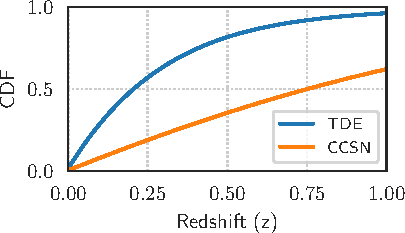
\includegraphics{bran/figure_s1_completeness.pdf}
	\caption{Cumulative distribution function (CDF) for TDE neutrino emission as a function of redshift, with the CCSN CDF plotted for comparison.}
	\label{fig:cdf}
\end{marginfigure}

It is clear that, for this negative source evolution, the vast majority of TDE neutrinos are expected to arrive from sources in the local universe. This statement is independent of both the overall level of TDE neutrino production and the absolute TDE rate. ZTF has, thus far, reported the detection of TDEs up to a maximum redshift 0.212 \cite{van_velzen_20}. If we simply assume that ZTF can routinely detect TDEs up to a redshift of 0.15, fully 40\% of the total population flux should come from ZTF-detected sources. We would thus require that at least 2.8\% of the astrophysical neutrino alerts are produced by TDEs, which is fully compatible with the stacking limit. TDE-neutrino associations can thus be detected even if the vast majority of the astrophysical neutrino flux is produced by other source classes. As is clear in Figure \ref{fig:cdf}, the large relative contribution of detectable TDEs to the population neutrino flux is in marked contrast to supernova-like populations which are dominated by distant sources \sidecite{ps_icecube_19}, so follow-up searches for TDEs are significantly more sensitive than for these other potential sources.

One further caveat introduced is that these stacking limits are derived under the assumptions of unbroken power laws which extend across a broad energy range (100 GeV - 10 PeV), where many additional neutrinos would be expected at lower energies.  However, for the case of neutrino spectra dominated by high-energy components (as expected for p$\gamma$ neutrino production), no such low-energy neutrinos would be expected, and these existing constraints would then be substantially weakened.

\section{Implications of AT2019dsg}

While the TDE-neutrino stacking analysis suggests that TDEs are not the dominant source of astrophysical neutrinos, the IC191001A-AT2019dsg association suggests that they may nonetheless contribute a subdominant component. Taken together, these two results would require TDEs as a population to contribute 3-39\% of the diffuse neutrino flux. As TDE discovery rates have increased substantially since the previous IceCube analysis \sidecite{van_velzen_20, 2019ICRC...36.1016S}, future searches will be able to study neutrino emission from TDEs with much greater sensitivity.

 Central Engine + new timescales

Of additional interest would be a new search for gamma-ray emission from TDEs which has so far not yet been observed \sidecite{tde_gamma}. For a pp neutrino production scenario, the associated gamma rays would however fall within the sensitive range of gamma-ray telescopes, so this scenario could be securely identified through a joint neutrino-gamma ray signal. While no gamma-ray emission was measured using the \textit{Fermi}-LAT telescope for AT2019dsg, gamma-ray Cherenkov telescopes may be sensitive to the expected gamma-ray signal, and the corresponding low-energy (TeV) neutrino emission could confirm a hadronic origin. Conversely, the high optical depth of the UV photosphere would absorb any gamma rays accompanying p$\gamma$ neutrino emission \sidecite{2016PhRvD..93h3005W}. Some contribution from such gamma-dark sources is required to explain the large astrophysical neutrino flux \sidecite{2016PhRvL.116g1101M}.

The combination of gamma-ray and neutrino data would then provide an opportunity for multi-messenger analysis of TDEs. The detection of any gamma-rays would favour a pp neutrino production, while the measurement of O($\sim$1-10) TeV neutrinos without accompanying gamma rays would indicate that neutrino production is occurring in the X-ray photosphere rather than in the UV photosphere. Indeed, such a detection would confirm the presence of a hidden X-ray source in the first place, while our electromagnetic observations cannot. Conversely, a lack of complementary low-energy neutrinos and gamma rays implies that only UV photons serve as a target. Neutrinos can uniquely serve as probes of the inner region of TDEs, using this novel method of extragalactic neutrino tomography. 